\section{1変数関数の積分}
\subsection{積分とは何か}
この本を読んでいる読者の方々は,
``積分''というものに対していったいどんなイメージを抱いているだろうか? ある人は``積分とは微分の逆演算である''
といい,またある人は``積分とは面積を求めることだ''という.
``積分とは無限この足し算である''
という人もいるだろう.たった1つの技術なのに
どうしてこんなにも解釈の違いが出るのだろうか? 実は,これらの解釈はすべて正しいのである.
どういうことだろうか? 少し考えてみよう.

まずは積分の定義を知らなければならない.
数学も物理も,理論は定義から始まるのである.
\footnote{実は,理論はもう1段階低い階層から始まっている.
数学者は公理,物理学者は基本法則と呼んでいるものがそれである.}
積分には大きく分けて2種類あるのだが,
最初に定積分から片づけてしまおう.

\subsection{定積分}
$x$の関数$f(x)$を考えよう.各$x$に対し,$x$の微小変化$\mathrm{d}x$と$f(x)$との積$f(x) \: \mathrm{d}x$という量を考える.
$\mathrm{d}x$が微小なので,$f(x) \: \mathrm{d}x$の値も微小である.そして,この量を区間$[a, \, b]$のあらゆる場所にわたって
計算し,その総和をとる.この和のことを
$$
\int_a^b f(x) \: \mathrm{d}x
$$
と書き,これを関数$f(x)$の区間$[a, \, b]$における\emph{定積分}\index[widx]{ていせきぶん@定積分}と呼ぶ.
$\int$記号は``インテグラル''と読む.

実数$x$は,区間$[a, \, b]$内に無数に存在する.よって各$x$に対する$f(x) \: \mathrm{d}x$も無数に存在する.
その総和をとるのだから,積分とは無限個の足し算であるという解釈にはある程度の説得力がある.
足したいものの情報を$f(x)$に詰め込んでおくのである.$\mathrm{d}x$の分余計なものが紛れているが,
それは後で調整してやればいい.

この説明がもっとも端的に定積分の性質を表しており,応用上はこれだけ覚えておけば困ることはほとんどない.
関数の平均値を求めるときや,確率を考えるときにはこの解釈はとても役に立つ.
これらの話で積分が頻繁に使われるのは不可解というよりむしろ当然のことであろう.
積分を表す記号$\int$が和(Sum)の頭文字であるSを縦に引き伸ばした形をしているのはこういう事情からきているのである.
言葉や記号の定義は先人たちがわかりやすいようにうまくやっているのである.

また,$f(x) \: \mathrm{d}x$という量が何を表しているかといえば,縦の長さ$f(x)$,
横の長さ$\mathrm{d}x$の長方形の面積である.
$\mathrm{d}x$が微小なので,この長方形の面積は
曲線$y=f(x)$と,2直線$x=t$,$x=t+\mathrm{d}x$,
および$x$軸で囲まれる図形の面積とほぼ等しい.(図\ref{fig:sekibunmenseki})
これは,$x$の変化が微小なうちは$f(x)$はほとんど変化しないとみなすことができるからである.
\begin{figure}[h]
 \centering
 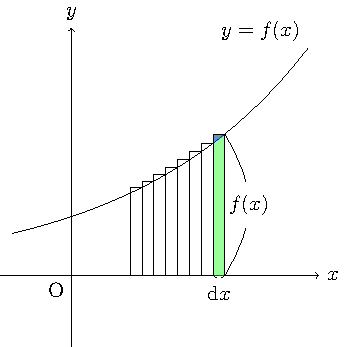
\includegraphics[width=5.5cm]{picture/sekibun1.pdf}
 \caption{積分は面積を表す}
  \label{fig:sekibunmenseki}
\end{figure}

$f(x) \: \mathrm{d}x$という部分が図の緑で塗った部分と青で塗った部分の面積の合計で,
``真の''面積が図の緑で塗った部分の面積である.
これらがほとんど違わないのがわかるだろう.もしも幅$\mathrm{d}x$をもっと小さくとれば,両者の差はもっと小さくなる. 
さらに,$\mathrm{d}x$を一種の理想的なごくごく微小な幅とすれば,もはや両者は完全に一致しているとみなしてよいだろう.
この小さい短冊状の図形の面積を区間$[a, \, b]$全域にわたって合計するのだ.
これが曲線$y=f(x)$,2直線$x=a$,$x=b$,および$x$軸で囲まれる図形の面積に等しいというのも納得がいくだろう.
ただし,$f(x)$は常に正の値をとるとは限らない.負の値をとることだって考えられる.
このとき,面積は負の値となってしまうので,定積分によって得られた値を
\emph{符号付き面積}\index[widx]{ふごうつきめんせき@符号付き面積}と呼ぶことにしよう.

これで定積分のおおまかなイメージはついただろう.``積分は微分の逆演算である''という解釈については何も説明してないが,
とりあえず後回しにさせてもらうことにして,定積分の正確な定義を書いておこう.
\subsubsection{定積分の正確な定義}
区間$[a, \, b]$で定義された有界な関数$f(x)$を考える.有界というのは大雑把に言えば
関数の値が途中で無限大に発散してしまうことはないくらいのイメージである.
和をとるときに無限大なんてものが混ざっていると足し算がうまくいかないので,そういう可能性を排除してあるのである.
そして,区間$[a, \, b]$を$n$個の小区間に分割するような分割$\varDelta$を考える.
\begin{equation*}
\varDelta : x_0 = a < x_1 < x_2 < \cdots < x_{n-1} < x_n =b
\end{equation*}
ここで重要なのが分割する,と言っているだけで等分とは一言も言っていない点である.どんな変な分割でもかまわない.
さらに,$\varDelta x_i = x_i - x_{i-1}$とおく.これは分割した各小区間の幅である.各小区間から点$c_i$を任意にとり,次のような和を考える.
\begin{equation*}
\sum_{i=1}^{n} f(c_i) \varDelta x_i
\label{riemannwa}
\end{equation*}
これがいわゆる$f(x)$の区間$[a, \, b]$における$f(x)$の\textbf{Riemann和}
\index[widx]{Riemannわ@Riemann和}
\index[nidx]{Riemann@Riemann(リーマン)}と呼ばれるものである.
ここで,各小区間の幅を限りなく小さくしてやる.
1つの式で書きたければ,$\varDelta x_i$の
最大値$\delta = \max \{ x_i-x_{i-1} \} $が限りなく小さくなるとでも書いてやればいい.
もちろん$n$が限りなく大きくなると考えても同じことである.
つまり,次のような極限を考えるのである.
\begin{equation*}
\lim_{\delta \to 0} \sum_{i=1}^{n} f(c_i) \varDelta x_i
\end{equation*}
この極限が分割$\varDelta$や$c_i$のとり方に依存せず,一定の値に確定するとき,関数$f(x)$は区間$[a, \, b]$で
\emph{可積分}\index[widx]{かせきぶん@可積分}であるといい,その極限値を
\begin{equation*}
\int_a^b f(x) \; \mathrm{d}x
\end{equation*}
と書く.そして,この極限値を求める操作を``定積分する''と呼ぶのである.

先ほどの直感的な説明とうまく対応しているのがわかるだろうか? $\Sigma$が$\int$に,
$\varDelta x_i$が$\mathrm{d}x$に,$c_i$が$x$に対応しているのである.

分割だの$c_i$だのは数学者が定義を正確にするために導入したいわば技巧的なものに過ぎない.
この技巧がどんなものかを学ぶことは非常に重要なことであるが,物理学の参考書という体裁上,
深入りするのはやめておくことにする.興味があれば勉強してみるのもいいだろう.

ただし,何が目的でこのような定義をしたかは知っておく必要がある.
この定義には面積などといった幾何学的な\footnote{ざっくりいうと図形的なという意味である.}要素は一切含まれていない.
面積はあくまで積分の解釈の1つに過ぎないのである.

そこで,面積というものを積分でもって定義することができるのである.
面積というものは今まであいまいなままであったが,これを積分でもって厳密に定義できるのである.
このあたりの話をもっと詳しく知るためには
$\varepsilon-\delta$論法を学ばなければならない.
後回しにすると面倒な理論なので興味があったら早めに学ぶとよい.
とっかかりは大変かもしれないが,そこから先は驚くほど単純である.
ただし,受験数学に毒されてしまった人にとっては難しいかもしれない.
\subsection{不定積分}
今までの説明では,積分と微分が互いに逆演算であるというイメージは出てこなかった.
積分とは無限個足し算であるという解釈なのであった.だが,そういう解釈をしたところで,
実際にそれを計算するのは非常に難しい.これでは積分はあまり役に立たない理論であったことだろう.
現実でそうなっていないのは微分と積分という一見関係なさそうに見える2つの概念が
実は深くかかわっていることが明らかになったからである.
この事実は微分積分学の基本定理
と呼ばれるもので,発見者はNewton\index[nidx]{Newton@Newton(ニュートン)}と
Leibniz\index[nidx]{Leibniz@Leibniz(ライプニッツ)}であり,互いに相手の研究内容は知らなかった. 
彼らが微分積分学の創始者であるといわれるのはこのことが理由になっているのである.
2人はほぼ同時期にこの定理を発見した.そのためかNewtonの支持者が
Leibnizをパクリだとひどく批判したが,Leibnizも自身の独創性を譲ろうとはしなかった.
もちろん微分積分学の理論は双方とも単独で作り上げたものであり,どちらがパクリなどということはない.

寄り道はこの辺にしておいて本題に戻るとしよう.定積分の話をするときに,積分には2種類あると言った.
1つはさっき説明した定積分であるが,
もう1つがこれから説明する不定積分である.

連続関数$f(x)$に対し,微分したら$f(x)$になるような関数$F(x)$があったとする.
\begin{eqnarray}
F'(x) = f(x)
\label{eq:ghuteisekibun}
\end{eqnarray}
ということである.この関数$F(x)$を$f(x)$の\emph{原始関数}\index[widx]{げんしかんすう@原始関数}と呼ぶ.
原始関数は無数に存在する.関数$f(x)$の原始関数$F(x)$が1つ存在すれば,それに定数$C$を加えた関数
$F(x)+C$も$f(x)$の原始関数だからである.これらをすべてまとめて
$$
\int f(x) \, \mathrm{d}x
$$
と書き,これを$f(x)$の\emph{不定積分}\index[widx]{ふていせきぶん@不定積分}と呼ぶ.
\begin{eqnarray}
\int f(x) \, \mathrm{d}x = F(x) + C \;\; (\text{ただし} F'(x)=f(x))
\label{eq:huteisekibun}
\end{eqnarray}
ということである.定積分のときと記号が似通っているのは微分積分学の基本定理があるからである.
両者のイメージはまったくの別物であるということには注意しなければならない.
不定積分の計算法は普通の数学書であれば必ず載っているのだが,今の目的は積分とは何なのかを知ることにあるので
とっとと先に進むことにする.
微分と積分がつながっているという事実を述べたのが次の定理である.
\begin{itembox}[l]{微分積分学の基本定理}
$a$を定数,$f(x)$を連続関数として,$x$の関数
$$
\int_{a}^{x} f(x) \, \mathrm{d}x
$$
は$f(x)$の原始関数である.つまり,
$$
\frac{\mathrm{d}}{\mathrm{d}x}\int_{a}^{x} f(x) \, \mathrm{d}x = f(x)
$$
となる.
\end{itembox}
積分して微分したら元に戻ってくるということは,微分と積分が互いに逆の演算であると言わざるを得ないだろう.

微分積分学の基本定理は別の表現もできる.
\begin{itembox}[l]{微分積分学の基本定理の別表現}
連続関数$f(x)$の任意の原始関数$F(x)$に対し,
$$
\int_{a}^{b} f(x) \, \mathrm{d}x = F(b)-F(a)
$$
となる.
\end{itembox}
ここでは,これらの定理の証明はしない.厳密に,正確に理解したければやはり$\varepsilon - \delta$論法を学ばなければならないからだ.
定積分の解説の最後の部分で述べた疑問への回答がこの定理である.定積分をしたければ,対象の関数の原始関数
を求めてやり,その変化量を計算してやればよいということである.
原始関数を求めることはときどき非常に面倒なケースに出くわすことがあるが,それでも``無限個の足し算''を実行するよりも
はるかにマシである.

また,高校ではこれが定積分の定義として扱われている.無限個の足し算というものが高校の範囲ではうまく説明できないからであろう.
しかし,それでは積分の本質にたどり着くことはできない.
この定義でもあまり問題はないのだが,面積というものが相変わらずあいまいなままになってしまう.
大学での積分論がよく理解できないのはこのあたりの事情が原因になっているのだと思う.
定義が変われば混乱するのも当たり前である.
\footnote{もしかしたら,高校生の間には定義は``神様''が決めるもので,
変えることは許されないという雰囲気が蔓延しているのかもしれない.}

最後に1つ補足をしておく.私はさっきまでずっと``定積分と不定積分のイメージはまったく違うものである''
と言ってきたが,よくよく考えてみるとそうでもないのである.
定積分のところで$f(x) \, \mathrm{d} x$というものが出てきた.
この形式,どこかで見たことはないだろうか? なんと,
この量は$f(x)$の原始関数の微分になっているではないか!
$f(x)$の原始関数の1つを$F(x)$としてみれば,$F(x)$の微分は
\begin{align*}
\mathrm{d}F = F'(x) \, \mathrm{d}x = f(x) \, \mathrm{d} x
\end{align*}
であるからだ.
この量をある範囲にわたって足し合わせていくのが定積分であった.$\mathrm{d} F$を連続した区間$[ a, \, b ]$で
足し合わせてみれば,はしっこ以外の値は打ち消されあって結局$F(b) - F(a)$しか残らない.
このことを確かめるのは読者にゆだねることにしよう.けっこういろいろと仮定を敷いていることに気が付くはずだ.
例えば$F(x)$の値が急激に激しく変化することはないとかそういうものである.
そして,そうして無限個の足し算を実行した結果は$\int$記号を用いて
\begin{align*}
\int_{F(a)}^{F(b)} \, \mathrm{d} F
\end{align*}
と書くのであった.
\footnote{表記の都合上積分範囲が変わっているが,とりあえず気にしなくてよい.}
ここではこの結果が$F(b)-F(a)$であったから
\begin{align*}
\int_{F(a)}^{F(b)} \mathrm{d}F = F(b) -F(a)
\end{align*}
である.最後に$\mathrm{d}F$は$f(x) \, \mathrm{d} x$だったのでこれを代入すると
\begin{align*}
\int_a^b f(x) \, \mathrm{d}x = F(b) - F(a)
\end{align*}
という式が得られたことになる.
これは微分積分学の基本定理ではないか! 微分と積分はこういうロジックでつながっているのである.
もちろん,こんなものは証明と呼べるようなものではない.
``無限個の足し算''や``微小''などといった概念はもっと慎重に扱わなければならないものである.
多くの物理数学の本では,
そのなかで正しいことが数学者のたゆまぬ努力によって証明されたものだけを都合よく拾ってきているのである.
詳しく知りたければやはり,$\epsilon - \delta$論法を学ぶべきである.
